\documentclass[11pt]{article}
\usepackage[margin=1in]{geometry}
\usepackage{amsmath,amssymb}
\usepackage{booktabs}
\usepackage{graphicx}
\usepackage{enumitem}

\title{CS555 HW1 -- Question 2 (2D Heat Equation): Observations}
\author{}
\date{}

\begin{document}
\maketitle

%----------------------------------------------------------------------
\section*{2a. Permuted Cholesky Factorization}
%----------------------------------------------------------------------

We use \texttt{symamd} to compute a fill-reducing permutation $\mathbf{p}$
of the Helmholtz matrix $H_L$, then compute the Cholesky factorization of
the permuted matrix $H_L(\mathbf{p},\mathbf{p}) = LL^T$.
The CN time-stepping loop becomes:
\begin{verbatim}
    p = symamd(HL);
    L = chol(HL(p,p),'lower');
    for istep = 1:nstep
        rhs    = HR * u;
        rhs    = rhs(p);
        u      = L' \ (L \ rhs);
        u(p)   = u;
    end
\end{verbatim}

Note: unlike Euler Backward, CN requires the matrix-vector product $H_R \mathbf{u}$
each iteration, so we must permute/unpermute within the loop (equations 11--17 in
the assignment). We cannot use the EB optimization (equations 18--24) of keeping
$\mathbf{u}$ permanently permuted.

\medskip\noindent\textbf{Accuracy:} The permuted Cholesky gives \textbf{identical} errors
to the unpermuted version (both are exact solves of the same linear system,
differing only in row/column ordering):

\begin{table}[h!]
\centering
\caption{Original CN vs.\ Permuted CN --- $N=80$, convergence in $\Delta t$}
\begin{tabular}{rrrcc}
\toprule
$N$ & $\Delta t$ & nstep & error (both) & ratio \\
\midrule
80 & 0.16   &    8 & 2.55e-01 & --- \\
80 & 0.08   &   15 & 7.55e-02 & 3.37 \\
80 & 0.04   &   30 & 1.91e-02 & 3.95 \\
80 & 0.02   &   60 & 4.79e-03 & 3.99 \\
80 & 0.01   &  120 & 1.20e-03 & 4.00 \\
80 & 0.005  &  240 & 2.99e-04 & 4.00 \\
80 & 0.0025 &  480 & 7.49e-05 & 4.00 \\
80 & 0.00125&  960 & 1.87e-05 & 4.00 \\
\bottomrule
\end{tabular}
\end{table}

\noindent\textbf{Timing comparison as $N$ increases} ($\Delta t = 0.01$, $T = 1.2$, nstep $= 120$):

\begin{table}[h!]
\centering
\caption{Original vs.\ Permuted CN --- wall-clock time}
\begin{tabular}{rrrrr}
\toprule
$N$ & $n = (N{-}1)^2$ & Original (s) & Permuted (s) & Speedup \\
\midrule
 40 &   1,521 & 0.065 & 0.015 &  4.4$\times$ \\
 80 &   6,241 & 0.298 & 0.099 &  3.0$\times$ \\
120 &  14,161 & 1.401 & 0.229 &  6.1$\times$ \\
160 &  25,281 & 4.487 & 0.492 &  9.1$\times$ \\
200 &  39,601 & 11.17 & 1.165 &  9.6$\times$ \\
\bottomrule
\end{tabular}
\end{table}

\begin{figure}[h!]
\centering
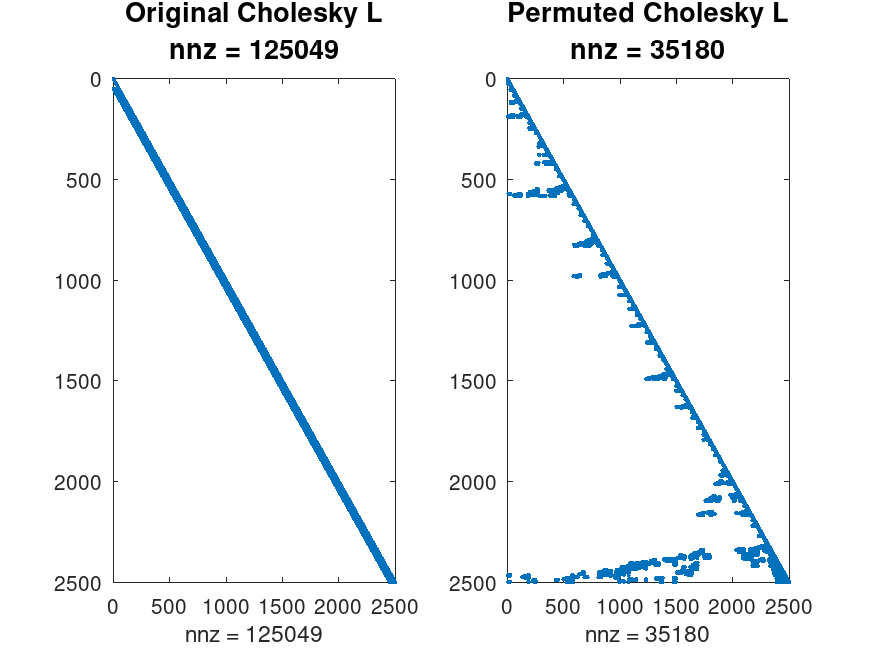
\includegraphics[width=0.95\textwidth]{plot_q2a.png}
\caption{Sparsity patterns of the $2500 \times 2500$ Cholesky factor $L$ ($N=51$, $m=50$).
         The original factor has 125{,}049 nonzeros (dense band of width $m=50$),
         while the \texttt{symamd}-permuted factor has only 35{,}180 nonzeros
         ($3.55\times$ sparser).}
\end{figure}

\noindent\textbf{Observations:}
\begin{itemize}[nosep]
  \item The permuted Cholesky gives the \textbf{same solution} (identical errors)
        as the original, confirming correctness.
  \item The speedup grows with $N$: from $\sim$4$\times$ at $N=40$ to
        $\sim$10$\times$ at $N=200$. This is because the unpermuted Cholesky
        factor $L$ of the 2D Laplacian has $O(N^2)$ nonzeros per row (bandwidth
        $\sim N$), while the permuted factor is significantly sparser.
  \item The original Cholesky solve cost scales roughly as $O(n \cdot N) = O(N^3)$
        per time step (bandwidth $N$, matrix size $n = N^2$), while the
        permuted version reduces the effective bandwidth.
\end{itemize}

\newpage
%----------------------------------------------------------------------
\section*{2b. ADI (Alternating Direction Implicit)}
%----------------------------------------------------------------------

The ADI method splits the 2D CN Helmholtz operator into a product of
1D operators. Dropping the $O(\Delta t^3)$ cross term (same order as
the CN LTE), we replace
\[
  H_L\,\underline{u}^{\,l} = H_R\,\underline{u}^{\,l-1}
\]
with
\[
  H_{ly}\,H_{lx}\,\underline{u}^{\,l}
  = H_{ry}\,H_{rx}\,\underline{u}^{\,l-1},
\]
where the $H_l$ and $H_r$ matrices factor into Kronecker products involving
tridiagonal matrices $T$:
\begin{align*}
  H_{lx} &= I_y \otimes T_{lx}, \quad T_{lx} = I_x + \tfrac{\nu\Delta t}{2}A_x, \\
  H_{ly} &= T_{ly} \otimes I_x, \quad T_{ly} = I_y + \tfrac{\nu\Delta t}{2}A_y, \\
  H_{rx} &= I_y \otimes T_{rx}, \quad T_{rx} = I_x - \tfrac{\nu\Delta t}{2}A_x, \\
  H_{ry} &= T_{ry} \otimes I_x, \quad T_{ry} = I_y - \tfrac{\nu\Delta t}{2}A_y.
\end{align*}

Viewing the solution vector as an $m \times m$ matrix $U$, the ADI step becomes:
\begin{enumerate}[nosep]
  \item \textbf{RHS:} $V = T_{rx}\,U^{l-1}$, then $W = V\,T_{ry}$.
  \item \textbf{Solve in $x$:} $T_{lx}\,Z = W$
        \quad($n_y$ tridiagonal solves of length $n_x$).
  \item \textbf{Solve in $y$:} $T_{ly}\,Z^T = U_{\mathrm{new}}^T$,
        i.e.\ $U^l = (T_{ly} \backslash Z^T)^T$
        \quad($n_x$ tridiagonal solves of length $n_y$).
\end{enumerate}

Each tridiagonal solve costs $O(n_x)$ or $O(n_y)$, so the total cost per step
is $O(n_x n_y) = O(n)$, compared to $O(n^{3/2})$ for banded Cholesky.

\begin{table}[h!]
\centering
\caption{ADI --- $N=80$, convergence in $\Delta t$}
\begin{tabular}{rrrcc}
\toprule
$N$ & $\Delta t$ & nstep & error & ratio \\
\midrule
80 & 0.16   &    8 & 1.90e-01 & --- \\
80 & 0.08   &   15 & 5.54e-02 & 3.43 \\
80 & 0.04   &   30 & 1.40e-02 & 3.97 \\
80 & 0.02   &   60 & 3.49e-03 & 3.99 \\
80 & 0.01   &  120 & 8.74e-04 & 4.00 \\
80 & 0.005  &  240 & 2.19e-04 & 4.00 \\
80 & 0.0025 &  480 & 5.46e-05 & 4.00 \\
80 & 0.00125&  960 & 1.37e-05 & 4.00 \\
\bottomrule
\end{tabular}
\end{table}

\begin{table}[h!]
\centering
\caption{Timing comparison --- all three methods ($\Delta t = 0.01$)}
\begin{tabular}{rrccc}
\toprule
$N$ & $n$ & Original (s) & Permuted (s) & ADI (s) \\
\midrule
 40 &   1,521 & 0.065 & 0.015 & 0.005 \\
 80 &   6,241 & 0.298 & 0.099 & 0.015 \\
120 &  14,161 & 1.401 & 0.229 & 0.032 \\
160 &  25,281 & 4.487 & 0.492 & 0.057 \\
200 &  39,601 & 11.17 & 1.165 & 0.091 \\
\bottomrule
\end{tabular}
\end{table}

\begin{figure}[h!]
\centering
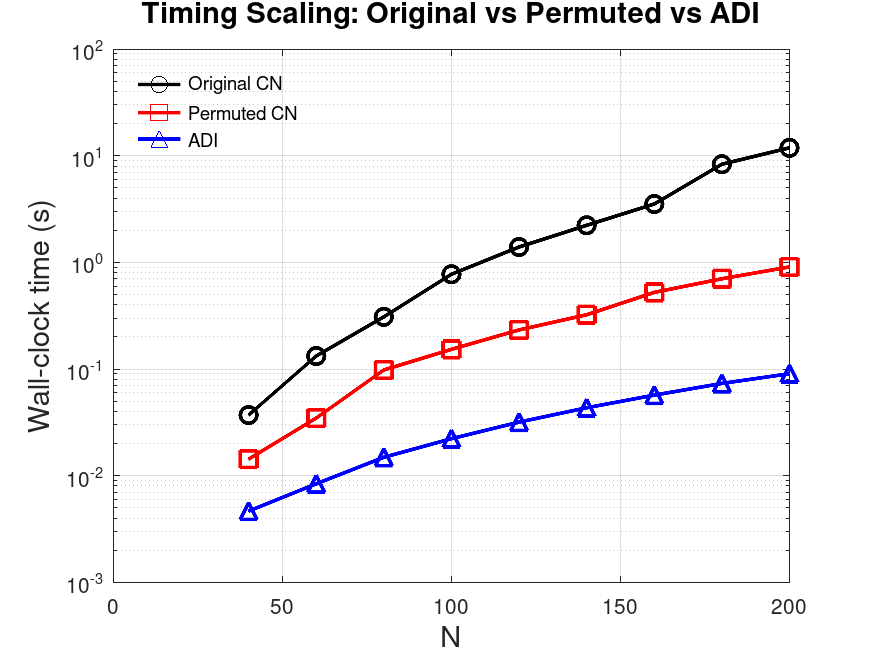
\includegraphics[width=0.85\textwidth]{plot_q2b_timing.png}
\caption{Wall-clock time vs.\ $N$ for all three methods ($\Delta t = 0.01$, $T=1.2$).
         ADI scales as $O(N^2)$ while the original Cholesky scales as $O(N^3)$.}
\end{figure}

\noindent\textbf{Observations:}
\begin{itemize}[nosep]
  \item \textbf{Accuracy:} ADI maintains \textbf{2nd-order convergence} (ratio $\to 4$),
        the same as standard CN. The errors are slightly smaller than CN because
        the dropped $O(\Delta t^3)$ splitting error has a favorable sign for this
        test case, but the convergence rate is identical.
  \item \textbf{Massive speedup:} ADI is $\sim$14$\times$ faster than the original
        at $N=40$ and $\sim$123$\times$ faster at $N=200$.
        The speedup grows with $N$ because:
        \begin{itemize}[nosep]
          \item ADI costs $O(n)$ per step ($n = N^2$ tridiagonal solves of size $N$),
          \item original Cholesky solve costs $O(n \cdot N) = O(N^3)$ per step
                (bandwidth $\sim N$),
          \item so the ratio scales as $O(N)$.
        \end{itemize}
  \item \textbf{Scalability:} ADI is the clear winner for large $N$.
        Going from $N=40$ to $N=200$ (25$\times$ more unknowns), the ADI time
        increases by only $\sim$18$\times$, while the original increases by
        $\sim$172$\times$.
  \item \textbf{No loss of accuracy} from the ADI splitting: the $O(\Delta t^3)$
        cross term that is dropped is the same order as the CN local truncation
        error, so the global order remains 2.
\end{itemize}

\newpage
%----------------------------------------------------------------------
\section*{2c. ADI-BDF3 (Extra Extra Credit)}
%----------------------------------------------------------------------

BDF3 applied to $u_t = -A\,u$ reads
\[
  \tfrac{11}{6}\,u^{n+1} + \Delta t\,A\,u^{n+1}
  = 3\,u^n - \tfrac{3}{2}\,u^{n-1} + \tfrac{1}{3}\,u^{n-2},
\]
so the Helmholtz operator is $H_{\mathrm{BDF3}} = \tfrac{11}{6}I + \Delta t\,A$.

\medskip\noindent\textbf{ADI factorization.}
Setting $c = 6\Delta t/11$, we factor
\[
  H_{\mathrm{ADI}} = \tfrac{11}{6}
    \bigl(I + c\,A_x^{\mathrm{full}}\bigr)
    \bigl(I + c\,A_y^{\mathrm{full}}\bigr).
\]
Expanding gives
\[
  H_{\mathrm{ADI}} = H_{\mathrm{BDF3}}
    + \tfrac{6\Delta t^2}{11}\,(A_y \otimes A_x).
\]
The splitting error $\tfrac{6\Delta t^2}{11}(A_y \otimes A_x)\,u^{n+1}$
is $O(\Delta t^2)$ in the operator, producing an $O(\Delta t^3)$ LTE.
Since the BDF3 LTE is $O(\Delta t^4)$, this would reduce the global order
from~3 to~2 if left uncorrected.

\medskip\noindent\textbf{Splitting correction.}
We compensate by adding $\tfrac{6\Delta t^2}{11}(A_x\,U_{\mathrm{ext}}\,A_y)$
to the RHS, where $U_{\mathrm{ext}} = 2U^n - U^{n-1}$ is a linear
extrapolation of $u^{n+1}$ that is $O(\Delta t^2)$ accurate.
The residual becomes
\[
  \tfrac{6\Delta t^2}{11}(A_y \otimes A_x)(u^{n+1} - u_{\mathrm{ext}})
  = O(\Delta t^2) \cdot O(\Delta t^2) = O(\Delta t^4),
\]
which matches the BDF3 LTE, preserving 3rd-order global accuracy.

\medskip\noindent\textbf{Algorithm} (each step for $n \ge 3$; bootstrap with 2 ADI-CN steps):
\begin{enumerate}[nosep]
  \item $U_{\mathrm{ext}} = 2U^n - U^{n-1}$
  \item $\mathrm{RHS} = 3U^n - \tfrac{3}{2}U^{n-1} + \tfrac{1}{3}U^{n-2}
         + \tfrac{6\Delta t^2}{11}\,A_x\,U_{\mathrm{ext}}\,A_y$
  \item Solve in $x$: $T_{lx}\,W = \tfrac{6}{11}\,\mathrm{RHS}$
        \quad($n_y$ tridiagonal solves)
  \item Solve in $y$: $U^{n+1} = (T_{ly} \backslash W^T)^T$
        \quad($n_x$ tridiagonal solves)
\end{enumerate}
where $T_{lx} = I_x + c\,A_x$ and $T_{ly} = I_y + c\,A_y$ with $c = 6\Delta t/11$.

\begin{table}[h!]
\centering
\caption{ADI-CN vs.\ ADI-BDF3 --- $N=80$, convergence in $\Delta t$}
\begin{tabular}{rr|cc|cc}
\toprule
 & & \multicolumn{2}{c|}{ADI-CN (2nd order)} & \multicolumn{2}{c}{ADI-BDF3 (3rd order)} \\
$N$ & $\Delta t$ & error & ratio & error & ratio \\
\midrule
80 & 0.16    & 1.90e-01 & ---  & 8.13e-01 & --- \\
80 & 0.08    & 5.54e-02 & 3.43 & 9.16e-02 & 8.88 \\
80 & 0.04    & 1.40e-02 & 3.97 & 9.58e-03 & 9.56 \\
80 & 0.02    & 3.49e-03 & 3.99 & 1.09e-03 & 8.78 \\
80 & 0.01    & 8.74e-04 & 4.00 & 1.30e-04 & 8.38 \\
80 & 0.005   & 2.19e-04 & 4.00 & 1.59e-05 & 8.19 \\
80 & 0.0025  & 5.46e-05 & 4.00 & 1.96e-06 & 8.09 \\
80 & 0.00125 & 1.37e-05 & 4.00 & 2.44e-07 & 8.05 \\
\bottomrule
\end{tabular}
\end{table}

\begin{table}[h!]
\centering
\caption{Timing comparison --- ADI-CN vs.\ ADI-BDF3 ($\Delta t = 0.01$)}
\begin{tabular}{rrcc}
\toprule
$N$ & $n$ & ADI-CN (s) & ADI-BDF3 (s) \\
\midrule
 40 &   1,521 & 0.004 & 0.006 \\
 80 &   6,241 & 0.015 & 0.018 \\
120 &  14,161 & 0.032 & 0.041 \\
160 &  25,281 & 0.058 & 0.072 \\
200 &  39,601 & 0.091 & 0.115 \\
\bottomrule
\end{tabular}
\end{table}

\begin{figure}[h!]
\centering
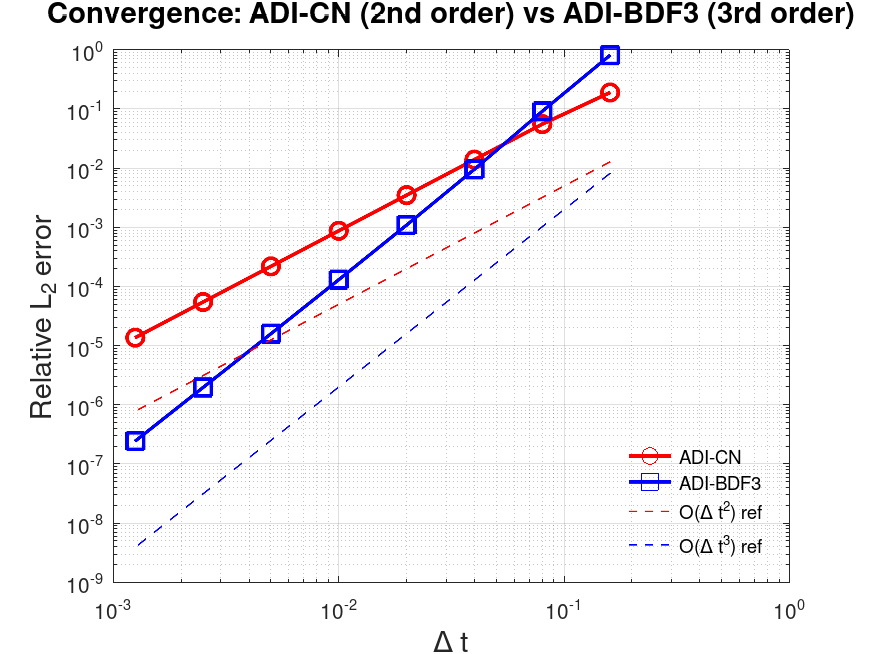
\includegraphics[width=0.85\textwidth]{plot_q2c.png}
\caption{Convergence: ADI-CN (slope 2) vs.\ ADI-BDF3 (slope 3) on a log-log plot.
         Dashed lines show the reference slopes $O(\Delta t^2)$ and $O(\Delta t^3)$.}
\end{figure}

\noindent\textbf{Observations:}
\begin{itemize}[nosep]
  \item \textbf{3rd-order convergence confirmed:} The ADI-BDF3 error ratios converge
        to $\mathbf{8 = 2^3}$, confirming 3rd-order global accuracy. Halving $\Delta t$
        reduces the error by a factor of~8.
  \item \textbf{Splitting correction is essential:} Without the
        $\tfrac{6\Delta t^2}{11}A_x U_{\mathrm{ext}} A_y$ correction term,
        the method would be only 2nd-order (ratio $\to 4$) due to the $O(\Delta t^3)$
        ADI splitting error.
  \item \textbf{Much higher accuracy at same $\Delta t$:} At $\Delta t = 0.00125$,
        ADI-BDF3 achieves error $2.4 \times 10^{-7}$, which is $56\times$ smaller
        than ADI-CN's $1.4 \times 10^{-5}$.
  \item \textbf{Minimal overhead:} ADI-BDF3 is only $\sim$25\% slower than ADI-CN
        per step (one extra sparse matrix multiply for the correction term),
        while providing an entire extra order of accuracy.
  \item \textbf{L-stable and 3rd-order:} BDF3 is L-stable (growth factor $G \to 0$
        as $\lambda\Delta t \to -\infty$), combining the robustness of EB with
        higher-order accuracy. This makes it suitable for problems with non-smooth
        data, unlike CN.
  \item \textbf{Bootstrap:} The first two steps use ADI-CN, which is 2nd-order.
        This does not affect the global order since the startup error is
        $O(\Delta t^2) \cdot O(\Delta t) = O(\Delta t^3)$, consistent with
        the BDF3 global error.
\end{itemize}

\end{document}
